\documentclass[conference]{IEEEtran}
\usepackage{graphicx,booktabs,amsmath,amssymb,url,xcolor,multirow}
\usepackage[hidelinks]{hyperref}
% auto-generated by scripts/make_paper.py -- do not edit
\newcommand{\MtlAllSharpe}{0.77}
\newcommand{\MtlAllCagr}{20.9\%}
\newcommand{\MtlAllMdd}{-27.7\%}
\newcommand{\MtlAllWin}{56.3\%}
\newcommand{\MtlAllPf}{1.49}
\newcommand{\MtlAllIc}{0.008}
\newcommand{\MtlAllIr}{0.99}
\newcommand{\MtlAllSortino}{1.31}
\newcommand{\MtlAllCalmar}{0.76}
\newcommand{\MtlAllWeeks}{167}
\newcommand{\MtlAllSharpeCi}{[-0.43, 1.92]}
\newcommand{\NoGraphAllSharpe}{0.44}
\newcommand{\NoGraphAllCagr}{14.4\%}
\newcommand{\NoGraphAllMdd}{-33.9\%}
\newcommand{\NoGraphAllWin}{51.5\%}
\newcommand{\NoGraphAllPf}{1.30}
\newcommand{\NoGraphAllIc}{0.005}
\newcommand{\NoGraphAllIr}{0.61}
\newcommand{\NoGraphAllSortino}{0.87}
\newcommand{\NoGraphAllCalmar}{0.43}
\newcommand{\NoGraphAllWeeks}{167}
\newcommand{\NoGraphAllSharpeCi}{[-0.71, 1.55]}
\newcommand{\MomAllSharpe}{0.06}
\newcommand{\MomAllCagr}{6.2\%}
\newcommand{\MomAllMdd}{-27.6\%}
\newcommand{\MomAllWin}{53.3\%}
\newcommand{\MomAllPf}{1.17}
\newcommand{\MomAllIc}{0.004}
\newcommand{\MomAllIr}{0.06}
\newcommand{\MomAllSortino}{0.09}
\newcommand{\MomAllCalmar}{0.22}
\newcommand{\MomAllWeeks}{167}
\newcommand{\MomAllSharpeCi}{[-1.08, 1.25]}
\newcommand{\InvVolAllSharpe}{0.11}
\newcommand{\InvVolAllCagr}{7.1\%}
\newcommand{\InvVolAllMdd}{-16.1\%}
\newcommand{\InvVolAllWin}{56.9\%}
\newcommand{\InvVolAllPf}{1.22}
\newcommand{\InvVolAllIc}{-0.030}
\newcommand{\InvVolAllIr}{0.14}
\newcommand{\InvVolAllSortino}{0.15}
\newcommand{\InvVolAllCalmar}{0.44}
\newcommand{\InvVolAllWeeks}{167}
\newcommand{\InvVolAllSharpeCi}{[-0.86, 1.07]}
\newcommand{\RandAllSharpe}{0.08}
\newcommand{\RandAllCagr}{6.8\%}
\newcommand{\RandAllMdd}{-24.0\%}
\newcommand{\RandAllWin}{52.9\%}
\newcommand{\RandAllPf}{1.20}
\newcommand{\RandAllIc}{--}
\newcommand{\RandAllIr}{0.10}
\newcommand{\RandAllSortino}{0.15}
\newcommand{\RandAllCalmar}{0.34}
\newcommand{\RandAllWeeks}{167}
\newcommand{\NiftyAllSharpe}{0.03}
\newcommand{\NiftyAllCagr}{6.1\%}
\newcommand{\NiftyAllMdd}{-15.5\%}
\newcommand{\NiftyAllWin}{55.1\%}
\newcommand{\NiftyAllPf}{1.22}
\newcommand{\NiftyAllIc}{--}
\newcommand{\NiftyAllIr}{--}
\newcommand{\NiftyAllSortino}{0.04}
\newcommand{\NiftyAllCalmar}{0.39}
\newcommand{\NiftyAllWeeks}{167}
\newcommand{\NiftyAllSharpeCi}{[-1.04, 1.08]}
\newcommand{\MtlTestSharpe}{2.54}
\newcommand{\MtlTestCagr}{74.9\%}
\newcommand{\MtlTestMdd}{-14.9\%}
\newcommand{\MtlTestWin}{70.5\%}
\newcommand{\MtlTestPf}{2.83}
\newcommand{\MtlTestIc}{0.064}
\newcommand{\MtlTestIr}{2.86}
\newcommand{\MtlTestSortino}{4.34}
\newcommand{\MtlTestCalmar}{5.02}
\newcommand{\MtlTestWeeks}{78}
\newcommand{\NoGraphTestSharpe}{2.01}
\newcommand{\NoGraphTestCagr}{61.5\%}
\newcommand{\NoGraphTestMdd}{-8.9\%}
\newcommand{\NoGraphTestWin}{65.4\%}
\newcommand{\NoGraphTestPf}{2.22}
\newcommand{\NoGraphTestIc}{0.037}
\newcommand{\NoGraphTestIr}{2.19}
\newcommand{\NoGraphTestSortino}{4.07}
\newcommand{\NoGraphTestCalmar}{6.94}
\newcommand{\NoGraphTestWeeks}{78}
\newcommand{\RetOnlyTestSharpe}{1.20}
\newcommand{\RetOnlyTestCagr}{28.0\%}
\newcommand{\RetOnlyTestMdd}{-8.6\%}
\newcommand{\RetOnlyTestWin}{53.8\%}
\newcommand{\RetOnlyTestPf}{1.76}
\newcommand{\RetOnlyTestIc}{0.017}
\newcommand{\RetOnlyTestIr}{0.85}
\newcommand{\RetOnlyTestSortino}{2.79}
\newcommand{\RetOnlyTestCalmar}{3.27}
\newcommand{\RetOnlyTestWeeks}{78}
\newcommand{\CostTestSharpe}{1.64}
\newcommand{\CostTestCagr}{41.9\%}
\newcommand{\CostTestMdd}{-15.6\%}
\newcommand{\CostTestWin}{61.5\%}
\newcommand{\CostTestPf}{2.05}
\newcommand{\CostTestIc}{0.031}
\newcommand{\CostTestIr}{1.65}
\newcommand{\CostTestSortino}{3.09}
\newcommand{\CostTestCalmar}{2.69}
\newcommand{\CostTestWeeks}{78}
\newcommand{\MomTestSharpe}{0.20}
\newcommand{\MomTestCagr}{8.7\%}
\newcommand{\MomTestMdd}{-22.2\%}
\newcommand{\MomTestWin}{56.4\%}
\newcommand{\MomTestPf}{1.22}
\newcommand{\MomTestIc}{0.018}
\newcommand{\MomTestIr}{-0.43}
\newcommand{\MomTestSortino}{0.28}
\newcommand{\MomTestCalmar}{0.39}
\newcommand{\MomTestWeeks}{78}
\newcommand{\InvVolTestSharpe}{0.99}
\newcommand{\InvVolTestCagr}{20.1\%}
\newcommand{\InvVolTestMdd}{-11.0\%}
\newcommand{\InvVolTestWin}{65.4\%}
\newcommand{\InvVolTestPf}{1.68}
\newcommand{\InvVolTestIc}{-0.048}
\newcommand{\InvVolTestIr}{0.49}
\newcommand{\InvVolTestSortino}{1.36}
\newcommand{\InvVolTestCalmar}{1.83}
\newcommand{\InvVolTestWeeks}{78}
\newcommand{\LogitTestSharpe}{2.20}
\newcommand{\LogitTestCagr}{54.1\%}
\newcommand{\LogitTestMdd}{-10.9\%}
\newcommand{\LogitTestWin}{64.1\%}
\newcommand{\LogitTestPf}{2.56}
\newcommand{\LogitTestIc}{0.026}
\newcommand{\LogitTestIr}{2.29}
\newcommand{\LogitTestSortino}{3.49}
\newcommand{\LogitTestCalmar}{4.97}
\newcommand{\LogitTestWeeks}{78}
\newcommand{\RandTestSharpe}{0.86}
\newcommand{\RandTestCagr}{20.7\%}
\newcommand{\RandTestMdd}{-14.5\%}
\newcommand{\RandTestWin}{59.2\%}
\newcommand{\RandTestPf}{1.59}
\newcommand{\RandTestIc}{--}
\newcommand{\RandTestIr}{0.44}
\newcommand{\RandTestSortino}{1.38}
\newcommand{\RandTestCalmar}{1.68}
\newcommand{\RandTestWeeks}{78}
\newcommand{\NiftyTestSharpe}{0.77}
\newcommand{\NiftyTestCagr}{15.5\%}
\newcommand{\NiftyTestMdd}{-10.1\%}
\newcommand{\NiftyTestWin}{64.1\%}
\newcommand{\NiftyTestPf}{1.58}
\newcommand{\NiftyTestIc}{--}
\newcommand{\NiftyTestIr}{--}
\newcommand{\NiftyTestSortino}{0.98}
\newcommand{\NiftyTestCalmar}{1.54}
\newcommand{\NiftyTestWeeks}{78}
\newcommand{\MtlHoldSharpe}{-1.12}
\newcommand{\MtlHoldCagr}{-12.4\%}
\newcommand{\MtlHoldMdd}{-25.9\%}
\newcommand{\MtlHoldWin}{43.8\%}
\newcommand{\MtlHoldPf}{0.77}
\newcommand{\MtlHoldIc}{-0.041}
\newcommand{\MtlHoldIr}{-0.88}
\newcommand{\MtlHoldSortino}{-1.69}
\newcommand{\MtlHoldCalmar}{-0.48}
\newcommand{\MtlHoldWeeks}{89}
\newcommand{\NoGraphHoldSharpe}{-1.08}
\newcommand{\NoGraphHoldCagr}{-15.4\%}
\newcommand{\NoGraphHoldMdd}{-33.9\%}
\newcommand{\NoGraphHoldWin}{39.3\%}
\newcommand{\NoGraphHoldPf}{0.76}
\newcommand{\NoGraphHoldIc}{-0.023}
\newcommand{\NoGraphHoldIr}{-1.08}
\newcommand{\NoGraphHoldSortino}{-1.97}
\newcommand{\NoGraphHoldCalmar}{-0.46}
\newcommand{\NoGraphHoldWeeks}{89}
\newcommand{\MomHoldSharpe}{-0.07}
\newcommand{\MomHoldCagr}{4.0\%}
\newcommand{\MomHoldMdd}{-16.6\%}
\newcommand{\MomHoldWin}{50.6\%}
\newcommand{\MomHoldPf}{1.13}
\newcommand{\MomHoldIc}{-0.009}
\newcommand{\MomHoldIr}{0.48}
\newcommand{\MomHoldSortino}{-0.12}
\newcommand{\MomHoldCalmar}{0.24}
\newcommand{\MomHoldWeeks}{89}
\newcommand{\InvVolHoldSharpe}{-0.54}
\newcommand{\InvVolHoldCagr}{-3.1\%}
\newcommand{\InvVolHoldMdd}{-15.6\%}
\newcommand{\InvVolHoldWin}{49.4\%}
\newcommand{\InvVolHoldPf}{0.95}
\newcommand{\InvVolHoldIc}{-0.014}
\newcommand{\InvVolHoldIr}{-0.11}
\newcommand{\InvVolHoldSortino}{-0.72}
\newcommand{\InvVolHoldCalmar}{-0.20}
\newcommand{\InvVolHoldWeeks}{89}
\newcommand{\RandHoldSharpe}{-0.57}
\newcommand{\RandHoldCagr}{-3.7\%}
\newcommand{\RandHoldMdd}{-16.6\%}
\newcommand{\RandHoldWin}{47.4\%}
\newcommand{\RandHoldPf}{0.95}
\newcommand{\RandHoldIc}{--}
\newcommand{\RandHoldIr}{-0.18}
\newcommand{\RandHoldSortino}{-0.90}
\newcommand{\RandHoldCalmar}{-0.19}
\newcommand{\RandHoldWeeks}{89}
\newcommand{\NiftyHoldSharpe}{-0.56}
\newcommand{\NiftyHoldCagr}{-1.6\%}
\newcommand{\NiftyHoldMdd}{-13.7\%}
\newcommand{\NiftyHoldWin}{47.2\%}
\newcommand{\NiftyHoldPf}{0.98}
\newcommand{\NiftyHoldIc}{--}
\newcommand{\NiftyHoldIr}{--}
\newcommand{\NiftyHoldSortino}{-0.94}
\newcommand{\NiftyHoldCalmar}{-0.12}
\newcommand{\NiftyHoldWeeks}{89}
\newcommand{\bestdropout}{0.3}
\newcommand{\bestlr}{0.0029}
\newcommand{\bestweightdecay}{0.00057}
\newcommand{\bestwreturn}{0.6}
\newcommand{\bestlambdaturnover}{0}
\newcommand{\besttargetmode}{raw}
\newcommand{\shapTopFive}{27\%}
\newcommand{\shapTopTen}{45\%}
\newcommand{\shapGraphShare}{75\%}
\newcommand{\attLastFour}{7\%}
\newcommand{\attLastTwelve}{20\%}
\newcommand{\attFirstTwelve}{20\%}
\newcommand{\topFeatureOne}{beta\_mkt}
\newcommand{\topFeatureTwo}{corr\_mkt}
\newcommand{\topFeatureThree}{pca\_3}
\newcommand{\topGroup}{graph\_corr}
\newcommand{\staticIcFinalVal}{0.067}
\newcommand{\staticIcFinalnographVal}{0.022}
\newcommand{\staticIcFinalretonlyVal}{-0.016}
\newcommand{\staticIcFinalsharpestopVal}{0.052}
\newcommand{\staticIcFinalTest}{0.046}
\newcommand{\staticIcFinalnographTest}{-0.025}
\newcommand{\staticIcFinalretonlyTest}{0.030}
\newcommand{\staticIcFinalsharpestopTest}{0.041}
\newcommand{\staticIcFinalHoldout}{-0.011}
\newcommand{\staticIcFinalnographHoldout}{-0.026}
\newcommand{\staticIcFinalretonlyHoldout}{-0.019}
\newcommand{\staticIcFinalsharpestopHoldout}{-0.000}
\newcommand{\sensCostZeroZeroZeroSide}{0.90}
\newcommand{\sensCostZeroZeroFiveSide}{0.83}
\newcommand{\sensCostZeroOneZeroSide}{0.77}
\newcommand{\sensCostZeroOneFiveSide}{0.70}
\newcommand{\sensCostZeroTwoFiveSide}{0.57}
\newcommand{\sensMaxPositionFive}{0.77}
\newcommand{\sensMaxPositionOneZero}{0.77}
\newcommand{\sensMaxPositionTwoZero}{0.77}
\newcommand{\sensModeRebalance}{0.77}
\newcommand{\sensModeHoldZone}{0.67}
\newcommand{\sensModeLongShort}{0.40}
\newcommand{\sensTopOneZeroOfUniverse}{0.77}
\newcommand{\sensTopTwoZeroOfUniverse}{0.55}
\newcommand{\sensDecisionERetEVolDefaultTest}{2.54}
\newcommand{\sensDecisionERetEVolDefaultHoldout}{-1.12}
\newcommand{\sensDecisionERetEVolDefaultAllOos}{0.77}
\newcommand{\sensDecisionERetOnlyTest}{2.26}
\newcommand{\sensDecisionERetOnlyHoldout}{-0.11}
\newcommand{\sensDecisionERetOnlyAllOos}{0.82}
\newcommand{\sensDecisionERetEVolZeroZeroThreeTest}{2.38}
\newcommand{\sensDecisionERetEVolZeroZeroThreeHoldout}{-0.21}
\newcommand{\sensDecisionERetEVolZeroZeroThreeAllOos}{0.95}
\newcommand{\sensDecisionEVolOnlyTest}{0.24}
\newcommand{\sensDecisionEVolOnlyHoldout}{-1.79}
\newcommand{\sensDecisionEVolOnlyAllOos}{-0.80}
\newcommand{\regMarketVolhighIc}{0.005}
\newcommand{\regMarketVolhighSharpe}{1.04}
\newcommand{\regMarketVollowIc}{0.011}
\newcommand{\regMarketVollowSharpe}{0.49}
\newcommand{\regAvgCorrelationhighIc}{-0.024}
\newcommand{\regAvgCorrelationhighSharpe}{0.75}
\newcommand{\regAvgCorrelationlowIc}{0.039}
\newcommand{\regAvgCorrelationlowSharpe}{0.78}
\newcommand{\regMarketOneTwoWTrendhighIc}{0.028}
\newcommand{\regMarketOneTwoWTrendhighSharpe}{1.50}
\newcommand{\regMarketOneTwoWTrendlowIc}{-0.012}
\newcommand{\regMarketOneTwoWTrendlowSharpe}{0.12}
\newcommand{\regDispersionhighIc}{0.014}
\newcommand{\regDispersionhighSharpe}{0.87}
\newcommand{\regDispersionlowIc}{0.002}
\newcommand{\regDispersionlowSharpe}{0.68}
\newcommand{\regMarketWeekbenchLtMinusTwoIc}{0.091}
\newcommand{\regMarketWeekbenchLtMinusTwoSharpe}{-12.58}
\newcommand{\regMarketWeekbenchGeMinusTwoIc}{-0.003}
\newcommand{\regMarketWeekbenchGeMinusTwoSharpe}{1.88}

% Results prose. Numbers come from numbers.tex macros where one exists; the few
% literal values are from results/tables/sensitivity.csv and failure_*.csv.

\newcommand{\RESULTSMAIN}{%
Over the full out-of-sample span the MTL strategy earns an annualized Sharpe ratio of \MtlAllSharpe{} (CAGR \MtlAllCagr, maximum drawdown \MtlAllMdd, weekly win rate \MtlAllWin, profit factor \MtlAllPf) with an information ratio of \MtlAllIr{} against the Nifty~50, which returned \NiftyAllCagr{} p.a.\ with a Sharpe of \NiftyAllSharpe{} over the same weeks. Every baseline that trades the same universe through the same engine is close to zero: momentum \MomAllSharpe, inverse volatility \InvVolAllSharpe, random 5-stock portfolios \RandAllSharpe. The graph-feature ablation retains part of the edge (\NoGraphAllSharpe) but with a deeper drawdown (\NoGraphAllMdd). Two caveats are visible in the same table. First, the 95\% block-bootstrap interval for the MTL Sharpe, \MtlAllSharpeCi, includes zero: 167 weeks of a five-stock portfolio cannot establish significance on their own. Second, the mean weekly rank-IC over the whole span is only \MtlAllIc, which is far smaller than the portfolio statistics suggest---the two disagree because, as the period breakdown shows next, the signal is concentrated in time.}

\newcommand{\RESULTSPERIODS}{%
Table~\ref{tab:periods} splits the span into the PRD test period (2023-H2 to 2024, \MtlTestWeeks{} weeks) and the untouched holdout (2025 to September~2026, \MtlHoldWeeks{} weeks). The two halves could hardly differ more. In the test period the strategy earns a Sharpe of \MtlTestSharpe{} (CAGR \MtlTestCagr, drawdown \MtlTestMdd, win rate \MtlTestWin, IC \MtlTestIc) while the Nifty~50 returned \NiftyTestCagr{} (Sharpe \NiftyTestSharpe); the quarterly rank-IC of the return head was 0.10, 0.10, 0.15 and 0.10 in the four quarters from 2023-Q3 to 2024-Q2, an unusually strong cross-sectional signal. In the holdout the strategy \emph{loses} money: Sharpe \MtlHoldSharpe, CAGR \MtlHoldCagr, IC \MtlHoldIc, against a flat market (Nifty CAGR \NiftyHoldCagr, Sharpe \NiftyHoldSharpe) in which momentum (\MomHoldSharpe) and random portfolios (\RandHoldSharpe) also fail. The calendar-year view in Table~\ref{tab:yearly} makes the transition explicit: the model beat the index by 31 and 51 percentage points in 2023-H2 and 2024, then trailed it by 15 points in 2025 and by 5 points in 2026. The rolling IC (Fig.~\ref{fig:rollic}) crosses zero in the third quarter of 2024 and never recovers. We return to why in Sec.~\ref{sec:limits}; the decile plot of Fig.~\ref{fig:decile} shows the pooled outcome: the top decile earns the highest mean weekly return, but the pattern across deciles is not monotone.}

\newcommand{\RESULTSABLATION}{%
Table~\ref{tab:ablation} compares the full model with its ablations on the PRD test period, where all variants were run (the return-only and cost-term variants were not extended into the holdout for compute reasons; the no-graph variant was). Removing the graph features lowers the test Sharpe from \MtlTestSharpe{} to \NoGraphTestSharpe{} and the IC from \MtlTestIc{} to \NoGraphTestIc; over the full span the gap is \MtlAllSharpe{} versus \NoGraphAllSharpe. Removing the volatility task is more damaging: a return-only model with the same backbone reaches only \RetOnlyTestSharpe{} (IC \RetOnlyTestIc) and trades far more (turnover 0.92 versus 0.36 per week), which is the clearest evidence in the study that the auxiliary volatility task regularizes the shared representation. Adding the transaction-cost term ($\lambda=0.3$) to the tuned configuration did \emph{not} help (\CostTestSharpe, IC \CostTestIc, turnover 0.69): the tuner had already rejected $\lambda>0$ on validation IC, and the softmax-implied portfolio used by the penalty is a poor proxy for the hard top-decile portfolio that is actually traded. The logistic-regression baseline on the same last-week and graph features is a strong competitor on the test period (\LogitTestSharpe, IC \LogitTestIc) at higher turnover (0.86); we did not run it on the holdout. The static single-fit models tell the same story in IC terms (val / test / holdout): full model \staticIcFinalVal{} / \staticIcFinalTest{} / \staticIcFinalHoldout; no-graph \staticIcFinalnographVal{} / \staticIcFinalnographTest{} / \staticIcFinalnographHoldout; return-only \staticIcFinalretonlyVal{} / \staticIcFinalretonlyTest{} / \staticIcFinalretonlyHoldout; and selecting the stopping epoch on validation Sharpe instead of IC gives \staticIcFinalsharpestopVal{} / \staticIcFinalsharpestopTest{} / \staticIcFinalsharpestopHoldout.}

\newcommand{\RESULTSSENS}{%
Table~\ref{tab:sens} and Fig.~\ref{fig:cost} vary the backtest assumptions on the full span. The strategy survives realistic costs: the Sharpe falls from 0.90 with free trading to 0.77 at the 0.1\%/side base case and 0.57 at 0.25\%/side, a slope consistent with its 0.47 average weekly one-way turnover. The hold-zone rule cuts turnover to 0.18 at a modest cost in Sharpe (0.67) and improves the drawdown (\(-23.4\%\)). A dollar-neutral long--short book is worse (0.40): the SELL decile carries little information beyond what the BUY decile already exploits, and shorting doubles the cost burden. Widening the BUY set to the top 20\% dilutes the edge (0.55). The 5\% position cap prescribed in the PRD leaves 75\% of capital in cash and therefore only rescales the CAGR (10.3\% versus 20.9\%); the Sharpe is unchanged because cash earns the risk-free rate. The last block of the table is a post-hoc diagnostic of the decision layer that we did not use for any selection: ranking on the predicted return alone would have delivered a Sharpe of 0.82 over the full span and \emph{flat} performance in the holdout (\(-0.11\), IC \(+0.014\)) instead of the \(-1.12\) obtained with $\hat r/\hat\sigma$; a shrunk ratio $\hat r/(\hat\sigma+0.03)$ sits in between (0.95 full span, \(-0.21\) holdout). Ranking on predicted volatility alone is strongly negative (\(-0.80\)). In other words, the Sharpe-style score is the right idea when the return forecast is informative, but when that forecast decays towards zero, dividing by volatility turns noise into a systematic tilt.}

\newcommand{\RESULTSATT}{%
The attention analysis produced a negative result that we consider informative. In the tuned model both the self-attention and the pooling weights are exactly uniform (entropy \(4.094\) versus \(\log 60 = 4.094\); the share on the last four weeks is \attLastFour, i.e.\ $4/60$). Inspection of the weights shows why: the selected weight decay (\bestweightdecay, roughly 57 times the PRD default of $10^{-5}$) shrinks the attention projection matrices to a norm of $10^{-3}$, so the sequence encoder degenerates into a mean over the 60 tokens followed by the feed-forward layers, and the model effectively becomes ``pooled own-history $+$ graph features''. The PRD-default configuration (weight decay $10^{-5}$) retains a non-trivial attention pattern (projection norm 10.0), shown in Fig.~\ref{fig:att}: the most recent 3--4 weeks and the oldest positions receive above-uniform attention in the last layer, and the pooling weights tilt towards the recent weeks in high-volatility regimes and away from them in calm regimes, although the magnitudes are small (maximum 0.021 against a uniform 0.017). The lag profile of SHAP mass (Fig.~\ref{fig:shaplag}) is likewise nearly flat (the last four weeks carry 5.7\% of sequence attribution, the oldest twelve 21\%). The honest summary is that, at this data size ($\approx$9{,}500 training windows), the optimizer found no value in modelling \emph{which} past weeks matter and the validation-selected model is closer to a well-regularized MLP than to a transformer.}

\newcommand{\RESULTSSHAP}{%
SHAP attributions of the decision score on 600 test-period samples (Fig.~\ref{fig:shap}) are dominated by graph features: fourteen of the fifteen most important inputs are graph features, led by \topFeatureOne, \topFeatureTwo{} and \topFeatureThree, and the graph groups together account for \shapGraphShare{} of attribution mass (67\% if sequence attributions are aggregated by absolute value over lags rather than net). The correlation-trend group (betas, market and sector correlations) is the largest single group, followed by the market-regime descriptors and peer momentum. Importance is spread out: the five largest features explain \shapTopFive{} of the total and the ten largest \shapTopTen, so the PRD's target of ``top five features explain 60\%'' is not met. The direction of the largest effects is consistent with the failure analysis below: high market beta and high market correlation raise the score, i.e.\ the model learned to buy high-beta, market-sensitive names, which is exactly what worked in the 2023--2024 rally and stopped working afterwards.}

\newcommand{\RESULTSFAIL}{%
Table~\ref{tab:regimes} and Fig.~\ref{fig:regimes} condition the out-of-sample weeks on regime variables. The signal is clearly better when pairwise correlations are low (IC 0.039, $t=1.8$) than when they are high (\(-0.024\)), and in rising markets (12-week trend above median: IC 0.028, portfolio Sharpe 1.50) than in falling ones (\(-0.012\), 0.12); market volatility and dispersion make little difference. In the 19 weeks in which the index fell by more than 2\% the cross-sectional IC is actually high (0.091) but the long-only portfolio loses heavily (mean \(-2.5\%\) per week), i.e.\ the model ranks stocks sensibly inside a crash but cannot avoid the crash. By stock characteristic, BUY signals on high-beta names had the best hit rate (57\%, mean next-week return \(+1.1\%\)) against 46\% for low-beta names; IT stocks were the worst sector (hit rate 40\%, mean \(-1.3\%\)) and financial services the best (58\%). A final failure mode is procedural: with a 26-week validation window the IC-based early-stopping criterion sometimes selected the first epoch (in 4 of 39 seed-fold fits), so several folds are trained models in name only; seed averaging mitigates but does not remove this.}

\newcommand{\RESULTSDISC}{%
\textbf{What worked.} The volatility head is robust: its rank-IC against realized next-week volatility stays between 0.18 and 0.38 in every quarter, including the holdout (mean 0.26), and it beats the naive ``last week's volatility'' forecast in every split. Its presence improves the return head (return-only ablation) and halves turnover. The graph features carry most of the attribution mass and their removal costs performance in every period. And the system as specified---weekly decile portfolio, 0.1\% costs, walk-forward retraining---delivered a large, cost-robust edge for eighteen months.

\textbf{What did not.} The return signal is regime-bound. Its quarterly IC exceeded 0.10 throughout the 2023--2024 rally, during which the model's picks carried twice the 12-week momentum of the universe, and it fell to zero or below from 2024-Q3 onward while the model's picks lost their momentum tilt; the 2025--2026 holdout, a flat-to-down market, is where a strategy built on beta, correlation and momentum features should be expected to fail, and it did. The decision layer amplified the failure: dividing a near-zero return forecast by predicted volatility produced a systematic tilt with a significantly negative IC, whereas ranking on the return alone would have been flat. We report the holdout precisely because it is where the PRD targets (Sharpe $>1$, win rate $>52\%$) are missed; on the PRD test period alone they are exceeded by a wide margin (\MtlTestSharpe, \MtlTestWin).

\textbf{Methodological lessons.} (i)~Selecting on a 26-week validation Sharpe is close to selecting on noise (Fig.~\ref{fig:curves}); rank-IC is better but still weak enough to pick epoch~1 in some folds, and a longer validation window or a smoothed criterion should be used. (ii)~Hyper-parameter search on a short window can silently disable a component: the tuned weight decay removed the attention path, so the architecture that is reported is not the architecture that was trained. (iii)~One diagnostic during development (an IC computation for an untuned model) did look at the 2023-H2--2024 period; the holdout was never inspected, and it is the only period we regard as a clean test. (iv)~The differentiable cost term as formulated did not transfer to the hard top-decile portfolio; a penalty on the change in \emph{ranks}, or direct optimization of the traded portfolio's net return, is the natural next step. (v)~A model of this kind should be paired with a regime gate---the low-correlation / rising-trend conditions under which the signal has positive IC are observable at decision time.}

\newcommand{\RESULTSCONC}{%
On the PRD test period the system exceeded every target (Sharpe \MtlTestSharpe, win rate \MtlTestWin, information ratio \MtlTestIr); on the untouched 2025--2026 holdout it lost money (Sharpe \MtlHoldSharpe) as its beta- and momentum-driven return signal decayed and the Sharpe-style decision rule amplified the resulting noise; over the full span it remains ahead of every baseline (Sharpe \MtlAllSharpe{} against \NiftyAllSharpe{} for the index) but not significantly so.}


\title{Multi-Task Deep Learning with Graph Features for Risk-Adjusted Stock Selection in Emerging Markets}

\author{\IEEEauthorblockN{Pratik Shah}
\IEEEauthorblockA{Independent Researcher\\ Email: studentplanchahiye@gmail.com}}

\begin{document}
\maketitle

\begin{abstract}
Predicting absolute equity returns is notoriously difficult; predicting \emph{risk-adjusted} relative performance is a more tractable and more useful target for portfolio construction. We present a multi-task learning (MTL) model that jointly forecasts next-week return and next-week realized volatility for Nifty~50 constituents from a 60-week history processed by a two-layer self-attention encoder, augmented with 30 \emph{graph features} extracted from a weekly re-estimated stock--stock correlation network (PCA embeddings, peer momentum, correlation trends, eigenvector centrality and market-regime descriptors). Stocks are ranked by the Sharpe-like score $\hat{r}/\hat{\sigma}$; the top decile is bought and the bottom decile sold. Transaction costs enter the training objective through a differentiable turnover penalty on softmax-implied portfolio weights. In a walk-forward evaluation (retraining every 13 weeks, 0.1\% cost per side) over \MtlAllWeeks{} out-of-sample weeks from July~2023 to September~2026, the strategy achieves an annualized Sharpe ratio of \MtlAllSharpe{} (block-bootstrap 95\% CI \MtlAllSharpeCi) against \NiftyAllSharpe{} for the Nifty~50 and \MomAllSharpe{} for a momentum baseline. The result is strongly regime-dependent: on the pre-registered test period (2023-H2 to 2024) the Sharpe is \MtlTestSharpe{} with a mean weekly rank-IC of \MtlTestIc, whereas on an untouched 2025--2026 holdout the return signal decays and the strategy loses money (Sharpe \MtlHoldSharpe). Ablations show that the volatility task and the graph features both matter (return-only: \RetOnlyTestSharpe; no graph features: \NoGraphTestSharpe{} on the test period); the volatility head remains accurate in every quarter. SHAP attributes \shapGraphShare{} of the decision score to graph features, led by market beta and market correlation. We also document three methodological findings: model selection on a 26-week validation Sharpe is dominated by noise; the tuned weight decay silently disabled the attention path; and the Sharpe-style decision rule $\hat r/\hat\sigma$ amplifies noise once the return forecast weakens. All code, data scripts and results are released.
\end{abstract}

\begin{IEEEkeywords}
multi-task learning, attention, graph features, stock selection, Indian equities, backtesting, interpretability
\end{IEEEkeywords}

% =====================================================================
\section{Introduction}
The weak-form efficient market hypothesis leaves little room for forecasting individual stock returns from price history alone, and the empirical literature on deep learning for return prediction is dominated by results that fail to survive realistic transaction costs or honest out-of-sample evaluation. Three observations motivate a different formulation.

\textbf{Risk matters as much as return.} An investor ranks opportunities by risk-adjusted return, yet most learning systems regress the return alone; a stock with a large predicted return and enormous uncertainty is then recommended as confidently as a steady compounder. Jointly modelling return and volatility lets the decision layer rank on $\hat{r}/\hat{\sigma}$, and the volatility task---which is far more predictable than the return task because of volatility clustering---provides a strong auxiliary signal that regularizes a shared representation.

\textbf{Stocks are not independent.} Sector co-movement, common factor exposure and time-varying correlation structure carry information about a stock's near-term behaviour that its own price history does not. We encode this structure with features computed on a correlation \emph{graph} that is re-estimated every week: eigen-decomposition embeddings, peer (sector) momentum, correlation trends against major sectors and the market, network centrality and its change, and a set of market-regime descriptors.

\textbf{Costs must be part of the objective.} A weekly-rebalanced portfolio of a handful of names is a high-turnover strategy. Charging costs only in the backtest reports the damage; putting them in the loss function lets the model trade off signal strength against turnover.

We build a system around these ideas for the Indian large-cap market and evaluate it with a walk-forward protocol on data through September~2026, holding back 2025--2026 as a period that no design decision ever touched. Our contributions are: (i) a joint return--volatility attention model with a decision layer that ranks on predicted Sharpe; (ii) a family of graph features from a weekly correlation network and an ablation quantifying their value; (iii) a differentiable transaction-cost term inside the training objective; (iv) an interpretability study using attention and SHAP; and (v) an honest, reproducible evaluation including the finding that validation Sharpe on short windows is an unreliable model-selection criterion.

% =====================================================================
\section{Related Work}
\textbf{Stock prediction.} Classical approaches regress returns on technical indicators or accounting factors~\cite{fama1993,jegadeesh1993}. Deep sequence models (LSTM, temporal convolution, transformers) have been applied to daily prices~\cite{fischer2018,sezer2020}, with the recurring criticism that in-sample gains rarely translate to out-of-sample, cost-adjusted performance~\cite{gu2020}. Gu, Kelly and Xiu~\cite{gu2020} show that non-linear models add most value in the \emph{cross-section}, which motivates our cross-sectional ranking formulation and our optional cross-sectionally demeaned target.

\textbf{Multi-task learning in finance.} MTL~\cite{caruana1997,ruder2017} has been used to share representations across horizons or across assets~\cite{ma2021mtl}. Predicting volatility alongside return is natural because volatility is strongly autocorrelated~\cite{engle1982,bollerslev1986} and realized-volatility forecasting with intraday data is well established~\cite{andersen2003}; the auxiliary task acts as an inductive bias for the noisier primary task.

\textbf{Graphs in finance.} Correlation networks of equities exhibit sector structure, hubs and regime-dependent topology~\cite{mantegna1999,onnela2003}. Graph neural networks have been applied to stock prediction using industry or supply-chain relations~\cite{feng2019,chen2018}. We take a lighter route that keeps the model small and interpretable: we compute explicit graph statistics (embeddings, centrality, peer aggregates) and feed them as features, which also makes them directly attributable with SHAP.

\textbf{Interpretability.} Attention weights offer a coarse view of which inputs the model uses~\cite{vaswani2017}; SHAP~\cite{lundberg2017} provides additive attributions with respect to a background distribution. We use both on the decision score rather than on the raw regression outputs.

% =====================================================================
\section{Methodology}
\subsection{Problem formulation}
Let $\mathcal{U}$ be the universe of $N$ stocks and let weeks be indexed by their Friday close $t$. For every stock $i$ with a clean 60-week history at $t$ we form a sequence $X_{i,t}\in\mathbb{R}^{60\times F_s}$ of own-history features and a static vector $z_{i,t}\in\mathbb{R}^{F_z}$ of graph and sector features. The targets are the next-week log return $r_{i,t+1}=\log(P_{i,t+1}/P_{i,t})$ and the next-week realized volatility $\sigma_{i,t+1}=\sqrt{5}\,\mathrm{std}(\text{daily log returns in week }t{+}1)$, clipped to $[0.01,0.10]$. The model outputs $(\hat r,\hat\sigma)$ and the decision layer ranks stocks by $s_{i,t}=\hat r_{i,t}/\hat\sigma_{i,t}$: the top decile is BUY, the bottom decile SELL and the rest HOLD.

\subsection{Features}
\textbf{Own-history sequence ($F_s=31$).} For each of the 60 weeks: candle geometry relative to the previous close ($\log O/C_{-1}$, $\log H/C_{-1}$, $\log L/C_{-1}$, $\log C/C_{-1}$), log volume ratio to its 12-week mean, realized volatility; 15 technical indicators (RSI-14, MACD line/signal/histogram scaled by price, Bollinger \%B and width, ATR/price, normalized OBV, CCI-20, stochastic \%K/\%D, Williams \%R, ADX, $\pm$DI); and 10 statistical features (1/4/12/26-week returns, 4- and 12-week volatility, 12-week skewness, kurtosis, lag-1 autocorrelation, volume ratio).

\textbf{Graph features ($30$).} Every week we estimate the $N\times N$ correlation matrix $C_t$ of daily log returns over the trailing 63 trading days. (1)~\emph{PCA embedding} (5): each stock's loadings on the five leading eigenvectors of $C_t$, sign-aligned across weeks. (2)~\emph{Peer momentum} (5): sector-mean 1/4/12-week returns excluding the stock itself, relative strength vs.\ sector, and 10-week sector momentum. (3)~\emph{Correlation trends} (10): correlation with equal-weight Banks, IT and Energy indices and with the Nifty~50; change of market correlation between 63- and 126-day windows; 12-week volatility of the 21-day market correlation; average intra- and extra-sector correlation; market and sector betas. (4)~\emph{Network centrality} (5): eigenvector centrality of the non-negative correlation graph, degree centrality at $|\rho|>0.3$, 13-week change in eigenvector centrality, local clustering coefficient, sector-average centrality. (5)~\emph{Market regime} (5): 20-day market volatility, 12-week market return, deviation from the 26-week moving average, average pairwise correlation and cross-sectional return dispersion. Together with an 11-way sector one-hot this gives $F_z=41$.

All features at $t$ use only data up to the close of week $t$; a unit test perturbs every price after $t$ and asserts that features and targets at $\le t$ are bit-identical.

\subsection{Model}
\begin{figure}[t]\centering\scriptsize
\begin{tabular}{@{}rcl@{}}
$X_{i,t}\,[60{\times}31]$ & $\xrightarrow{\;\text{Linear}+\text{pos.\ emb.}\;}$ & $[60{\times}d]$ \\
 & $\xrightarrow{\;2\times(\text{MHA}_{8}+\text{FFN}),\ \text{pre-LN}\;}$ & $[60{\times}d]$ \\
 & $\xrightarrow{\;\text{learned-query attention pooling}\;}$ & $h_s\in\mathbb{R}^{d}$ \\[2pt]
$z_{i,t}\,[41]$ & $\xrightarrow{\;\text{Linear}+\text{GELU}\;}$ & $h_z\in\mathbb{R}^{d}$ \\[2pt]
$[h_s;h_z]$ & $\xrightarrow{\;\text{FC}(128)+\text{ReLU}+\text{Dropout}\;}$ & $h\in\mathbb{R}^{128}$ \\
$h$ & $\xrightarrow{\;\text{FC}(64)\to\text{FC}(1)\;}$ & $\hat r$ \quad (return head) \\
$h$ & $\xrightarrow{\;\text{FC}(64)\to\text{FC}(1)\;}$ & $\hat\sigma$ \quad (volatility head)
\end{tabular}
\caption{Architecture. $d=64$, 8 heads, two pre-LayerNorm blocks, dropout \bestdropout{} on residual and FFN paths, learned-query attention pooling whose weights are used for interpretation.}
\label{fig:arch}
\end{figure}
Figure~\ref{fig:arch} summarizes the network. The sequence is projected to $d$ dimensions, added to a learned positional embedding, and passed through two pre-LayerNorm self-attention blocks (8 heads) with GELU feed-forward sub-layers. A learned query attends over the 60 positions to produce a pooled vector, whose attention weights answer ``which past weeks matter''. The static vector is projected separately; the concatenation feeds a shared FC(128) backbone and two FC(64)$\to$1 task heads. Both heads predict in standardized target space; volatility is de-standardized and clipped to $[0.01,0.10]$ before use.

\subsection{Training objective}
With standardized targets $\tilde r,\tilde\sigma$ the loss for one weekly cross-section $B_t$ is
\begin{equation}
\mathcal{L}=w\,\mathrm{MSE}(\hat{\tilde r},\tilde r)+(1-w)\,\mathrm{MSE}(\hat{\tilde\sigma},\tilde\sigma)+\lambda\,\mathcal{L}_{\text{cost}},
\end{equation}
\begin{equation}
\mathcal{L}_{\text{cost}}=-\frac{1}{\sigma_r}\Big[\textstyle\sum_i \omega_{i,t}\,r_{i,t+1}-c\sum_i|\omega_{i,t}-\omega_{i,t-1}|\Big],
\end{equation}
where $\omega_{\cdot,t}=\mathrm{softmax}(s_{\cdot,t}/\tau)$ are soft long-only weights implied by the scores of the same stocks in weeks $t$ and $t{-}1$ (a second forward pass), $c=0.1\%$ is the one-way cost and $\tau=0.1$. $\mathcal{L}_{\text{cost}}$ is the negative net portfolio return, so gradients push the model towards scores whose implied portfolio earns more \emph{after} the cost of changing it. Batches are whole weekly cross-sections ($\approx$45--50 stocks) so that both $\mathcal{L}_{\text{cost}}$ and portfolio-level validation metrics are computable. We use Adam (lr \bestlr, weight decay \bestweightdecay), gradient clipping at 1.0, at most 200 epochs and early stopping with patience 20.

\subsection{Model selection and the validation-Sharpe pitfall}
The PRD for this system prescribed early stopping on the validation-period Sharpe ratio. The validation period (2023-H1) has 26 weeks and the portfolio holds 5 names, so that criterion has a standard error of roughly $\sqrt{52/26}\approx1.4$ Sharpe units: in our runs it swung between $-1.3$ and $+2.4$ from one epoch to the next while the loss changed smoothly (Fig.~\ref{fig:curves}). We therefore select on the mean weekly rank information coefficient (IC) between score and realized return, which uses all $\approx$48 stocks each week, and report the Sharpe-selected model as an ablation. Hyper-parameters ($d$, depth, dropout, learning rate, weight decay, task weight $w$, $\lambda$ and the return-target mode) were tuned with 24 Optuna TPE trials on validation IC. The architecture ($d=64$, two layers) was fixed as in the PRD. The selected configuration is dropout \bestdropout, learning rate \bestlr, weight decay \bestweightdecay, $w=\bestwreturn$, $\lambda=\bestlambdaturnover$ and the raw (not demeaned) return target.

\subsection{Portfolio construction and backtest}
At each Friday close the top 10\% of scored stocks are bought equal-weight (5 names, 20\% each; the PRD's 5\% cap is reported as a sensitivity), the bottom 10\% are sold if held, and positions are rebalanced weekly. Costs of 0.1\% per side are charged on $\sum_i|\omega^{\text{target}}_i-\omega^{\text{drifted}}_i|$, where drifted weights reflect the week's price moves; uninvested capital earns the weekly risk-free rate (6.5\% p.a.). We also report a lower-turnover \emph{hold-zone} variant (a held stock is kept while it stays in the top half of the ranking) and a dollar-neutral long--short variant.

\textbf{Walk-forward.} Prediction week blocks of 13 weeks start in July~2023. For block $k$ the validation set is the 26 weeks immediately preceding it and the training set is everything from January~2019 up to the validation start (expanding window); predictions from 3 seeds are averaged. All figures below are out-of-sample in this sense. We split the reporting into the PRD test period (2023-H2 to 2024) and an untouched holdout (2025-01 to 2026-09) that was never used for any design decision.

% =====================================================================
\section{Experiments}
\subsection{Data}
Daily OHLCV for the current 50 Nifty~50 constituents and the index from January~2017 to September~2026 were obtained from Yahoo Finance (split/dividend adjusted; the October~2025 Tata Motors demerger is back-adjusted manually). Bars are resampled to weekly Friday closes. Stocks are eligible in a week if the price exceeds INR~10, trailing-year average volume exceeds 100K shares/day, fewer than 10\% of sessions are missing and a full 60-week feature window exists; recently listed names (Eternal, Jio Financial, Max Healthcare) enter once they qualify. Using current constituents introduces survivorship bias, which we discuss in Sec.~\ref{sec:limits}. The panel has 495 weeks $\times$ 50 stocks with 19{,}005 usable samples.

\subsection{Baselines}
(i)~\emph{Nifty~50 buy-and-hold}; (ii)~\emph{Momentum}: score = trailing 4-week return; (iii)~\emph{Inverse volatility}: score $=-$trailing 4-week volatility; (iv)~\emph{Random}: 20 random 5-stock portfolios per week, averaged; (v)~\emph{Logistic regression}: $P(r_{t+1}>\text{median})$ on the same last-week and graph features, retrained on the same walk-forward schedule. Baselines (ii)--(v) are run through the identical backtest engine with the same costs.

\subsection{Main results}
\begin{table}[t]\centering\caption{Out-of-sample performance, July~2023--September~2026 (\MtlAllWeeks{} weeks), net of 0.1\%/side costs. Sharpe and IR are annualized; brackets are 95\% stationary block-bootstrap CIs; IC is the mean weekly Spearman correlation between score and realized return; Turn.\ is average weekly one-way turnover.}\label{tab:main}
\resizebox{\columnwidth}{!}{\begin{tabular}{lrrrrrrrr}
\toprule
Strategy & Sharpe & CAGR & MDD & Win & PF & IR & IC & Turn. \\
\midrule
\textbf{MTL (ours)} & 0.77 {\scriptsize[-0.43, 1.92]} & 20.9\% & -27.7\% & 56.3\% & 1.49 & 0.99 & 0.008 & 0.47 \\
MTL no-graph & 0.44 {\scriptsize[-0.71, 1.55]} & 14.4\% & -33.9\% & 51.5\% & 1.30 & 0.61 & 0.005 & 0.20 \\
Momentum & 0.06 {\scriptsize[-1.08, 1.25]} & 6.2\% & -27.6\% & 53.3\% & 1.17 & 0.06 & 0.004 & 1.01 \\
Inverse-vol & 0.11 {\scriptsize[-0.86, 1.07]} & 7.1\% & -16.1\% & 56.9\% & 1.22 & 0.14 & -0.030 & 1.10 \\
Random & 0.08 & 6.8\% & -24.0\% & 52.9\% & 1.20 & 0.10 & -- & -- \\
Nifty 50 & 0.03 {\scriptsize[-1.04, 1.08]} & 6.1\% & -15.5\% & 55.1\% & 1.22 & -- & -- & -- \\
\bottomrule
\end{tabular}
}\end{table}

\begin{figure}[t]\centering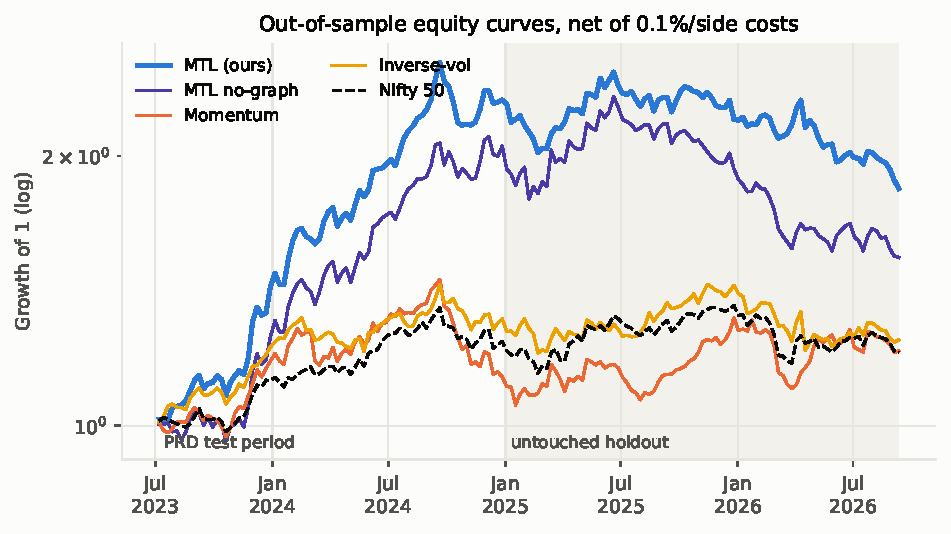
\includegraphics[width=\columnwidth]{figures/equity_curves.pdf}
\caption{Out-of-sample growth of one unit (log scale). The shaded region is the untouched 2025--2026 holdout.}\label{fig:equity}\end{figure}

Table~\ref{tab:main} and Fig.~\ref{fig:equity} report the full out-of-sample period. \RESULTSMAIN

\begin{table}[t]\centering\caption{Performance by period.}\label{tab:periods}\resizebox{\columnwidth}{!}{\begin{tabular}{llrrrrr}
\toprule
Period & Strategy & Sharpe & CAGR & MDD & Win & IC \\
\midrule
Test 2023-H2--2024 & MTL (ours) & 2.54 & 74.9\% & -14.9\% & 70.5\% & 0.064 \\
Test 2023-H2--2024 & Momentum & 0.20 & 8.7\% & -22.2\% & 56.4\% & 0.018 \\
Test 2023-H2--2024 & Logistic & 2.20 & 54.1\% & -10.9\% & 64.1\% & 0.026 \\
Test 2023-H2--2024 & Nifty 50 & 0.77 & 15.5\% & -10.1\% & 64.1\% & -- \\
Holdout 2025--2026 & MTL (ours) & -1.12 & -12.4\% & -25.9\% & 43.8\% & -0.041 \\
Holdout 2025--2026 & Momentum & -0.07 & 4.0\% & -16.6\% & 50.6\% & -0.009 \\
Holdout 2025--2026 & Nifty 50 & -0.56 & -1.6\% & -13.7\% & 47.2\% & -- \\
\bottomrule
\end{tabular}
}\end{table}
\begin{table}[t]\centering\caption{Calendar-year breakdown.}\label{tab:yearly}\resizebox{\columnwidth}{!}{\begin{tabular}{lrrrrr}
\toprule
Year & MTL return & Nifty return & MTL Sharpe & Nifty Sharpe & Weeks \\
\midrule
2023 & 43.2\% & 12.3\% & 3.18 & 1.68 & 26 \\
2024 & 61.4\% & 10.6\% & 2.19 & 0.37 & 52 \\
2025 & -4.9\% & 9.7\% & -0.60 & 0.30 & 52 \\
2026 & -16.3\% & -11.3\% & -1.92 & -1.66 & 37 \\
\bottomrule
\end{tabular}
}\end{table}

\RESULTSPERIODS

\begin{figure}[t]\centering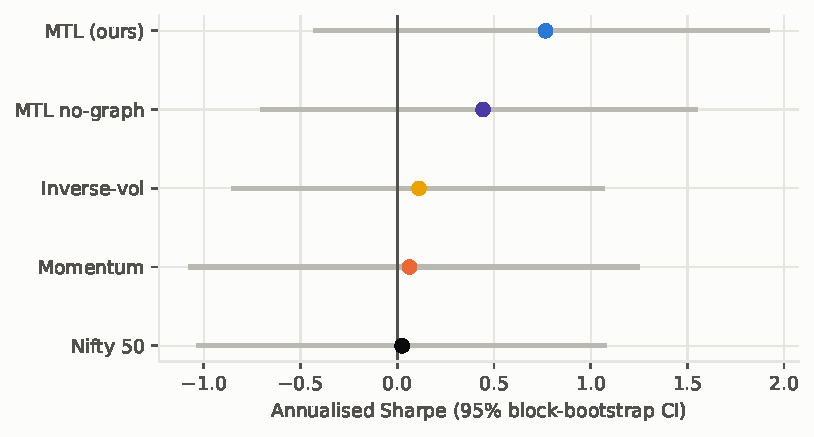
\includegraphics[width=\columnwidth]{figures/sharpe_ci.pdf}
\caption{Annualized Sharpe with 95\% block-bootstrap confidence intervals (all out-of-sample weeks).}\label{fig:ci}\end{figure}
\begin{figure}[t]\centering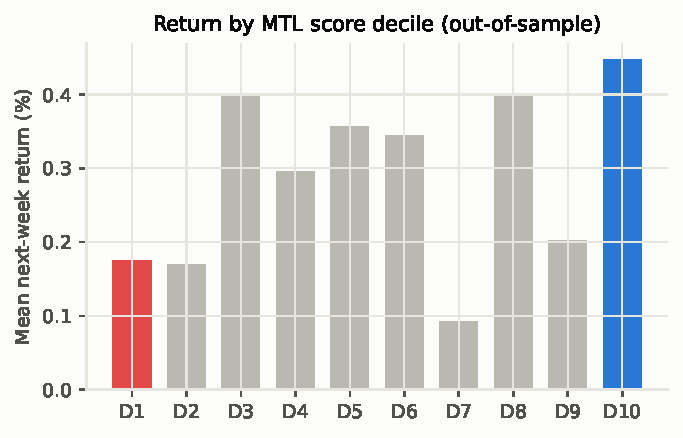
\includegraphics[width=0.85\columnwidth]{figures/decile_returns.pdf}
\caption{Mean realized next-week return by decile of the MTL score (D10 = highest score).}\label{fig:decile}\end{figure}

\subsection{Ablations}
\begin{table}[t]\centering\caption{Ablations on the PRD test period (2023-H2 to 2024, 78 weeks), net of costs.}\label{tab:ablation}\resizebox{\columnwidth}{!}{\begin{tabular}{lrrrrrr}
\toprule
Strategy & Sharpe & CAGR & MDD & Win & IC & Turn. \\
\midrule
\textbf{MTL (ours)} & 2.54 & 74.9\% & -14.9\% & 70.5\% & 0.064 & 0.36 \\
MTL no-graph & 2.01 & 61.5\% & -8.9\% & 65.4\% & 0.037 & 0.13 \\
MTL return-only & 1.20 & 28.0\% & -8.6\% & 53.8\% & 0.017 & 0.92 \\
MTL +cost-term & 1.64 & 41.9\% & -15.6\% & 61.5\% & 0.031 & 0.69 \\
Logistic & 2.20 & 54.1\% & -10.9\% & 64.1\% & 0.026 & 0.86 \\
Momentum & 0.20 & 8.7\% & -22.2\% & 56.4\% & 0.018 & 1.01 \\
Inverse-vol & 0.99 & 20.1\% & -11.0\% & 65.4\% & -0.048 & 1.07 \\
Random & 0.86 & 20.7\% & -14.5\% & 59.2\% & -- & -- \\
Nifty 50 & 0.77 & 15.5\% & -10.1\% & 64.1\% & -- & -- \\
\bottomrule
\end{tabular}
}\end{table}
\begin{figure}[t]\centering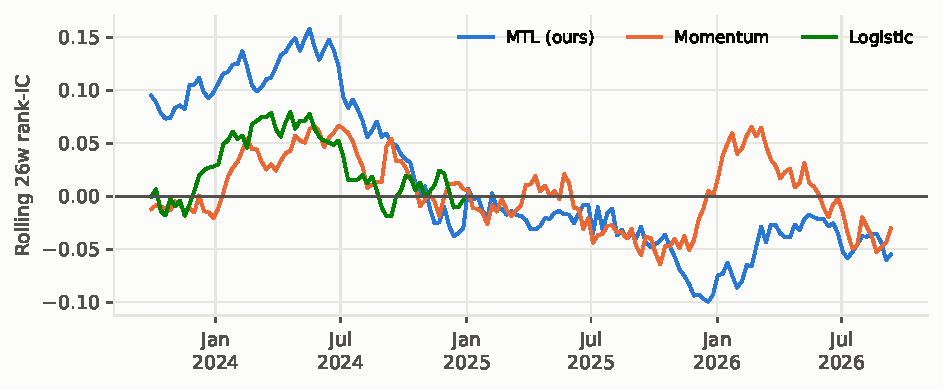
\includegraphics[width=\columnwidth]{figures/rolling_ic.pdf}\caption{Rolling 26-week rank-IC of the MTL score and two baselines.}\label{fig:rollic}\end{figure}
\RESULTSABLATION

\subsection{Sensitivity}
\begin{table}[t]\centering\caption{Sensitivity of the MTL strategy (all out-of-sample weeks).}\label{tab:sens}\resizebox{\columnwidth}{!}{\begin{tabular}{lrr}
\toprule
Setting & Sharpe & CAGR \\
\midrule
cost 0.00\%/side & 0.90 & 23.9\% \\
cost 0.05\%/side & 0.83 & 22.4\% \\
cost 0.10\%/side & 0.77 & 20.9\% \\
cost 0.15\%/side & 0.70 & 19.4\% \\
cost 0.25\%/side & 0.57 & 16.5\% \\
max position 5\% & 0.77 & 10.3\% \\
max position 10\% & 0.77 & 14.0\% \\
max position 20\% & 0.77 & 20.9\% \\
mode rebalance & 0.77 & 20.9\% \\
mode hold\_zone & 0.67 & 17.0\% \\
mode long\_short & 0.40 & 12.8\% \\
top 10\% of universe & 0.77 & 20.9\% \\
top 20\% of universe & 0.55 & 14.4\% \\
decision: $\hat r$/$\hat\sigma$ (default) {[}test{]} & 2.54 & 74.9\% \\
decision: $\hat r$/$\hat\sigma$ (default) {[}holdout{]} & -1.12 & -12.4\% \\
decision: $\hat r$/$\hat\sigma$ (default) {[}all\_oos{]} & 0.77 & 20.9\% \\
decision: $\hat r$ only {[}test{]} & 2.26 & 62.3\% \\
decision: $\hat r$ only {[}holdout{]} & -0.11 & 0.1\% \\
decision: $\hat r$ only {[}all\_oos{]} & 0.82 & 25.5\% \\
decision: $\hat r$/($\hat\sigma$+0.03) {[}test{]} & 2.38 & 67.6\% \\
decision: $\hat r$/($\hat\sigma$+0.03) {[}holdout{]} & -0.21 & -0.3\% \\
decision: $\hat r$/($\hat\sigma$+0.03) {[}all\_oos{]} & 0.95 & 27.0\% \\
decision: -$\hat\sigma$ only {[}test{]} & 0.24 & 9.1\% \\
decision: -$\hat\sigma$ only {[}holdout{]} & -1.79 & -16.7\% \\
decision: -$\hat\sigma$ only {[}all\_oos{]} & -0.80 & -5.5\% \\
\bottomrule
\end{tabular}
}\end{table}
\begin{figure}[t]\centering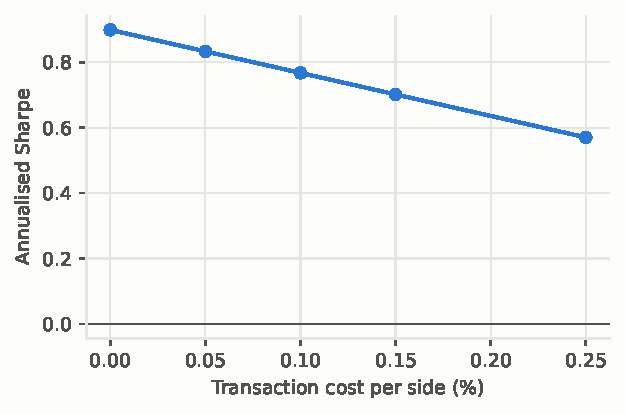
\includegraphics[width=0.8\columnwidth]{figures/cost_sensitivity.pdf}\caption{Annualized Sharpe versus one-way transaction cost.}\label{fig:cost}\end{figure}
\RESULTSSENS

% =====================================================================
\section{Interpretability Analysis}
\begin{figure}[t]\centering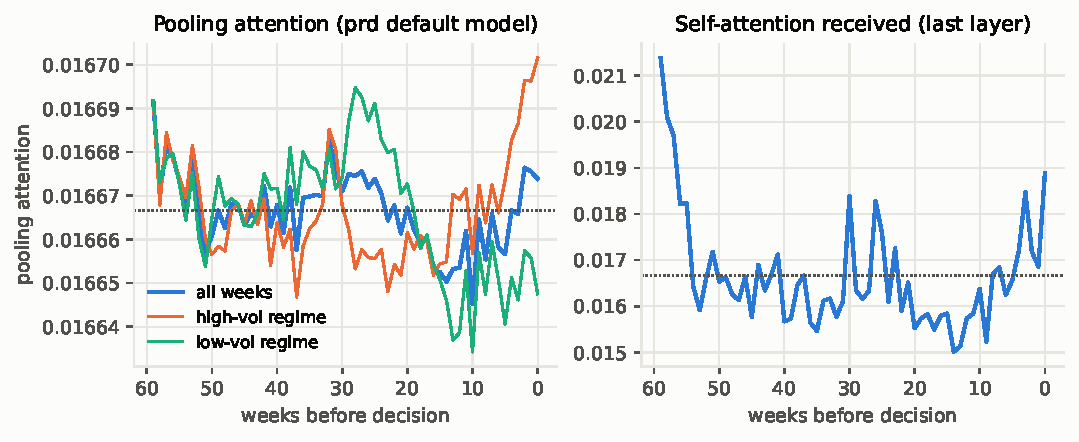
\includegraphics[width=\columnwidth]{figures/attention_by_lag.pdf}
\caption{Attention over the 60-week history on test-period samples for the PRD-default configuration (weight decay $10^{-5}$); the tuned model's attention is exactly uniform. Left: learned-query pooling weights, overall and split by market-volatility regime; dotted line is uniform. Right: self-attention received by each position in the last layer.}\label{fig:att}\end{figure}
\begin{figure}[t]\centering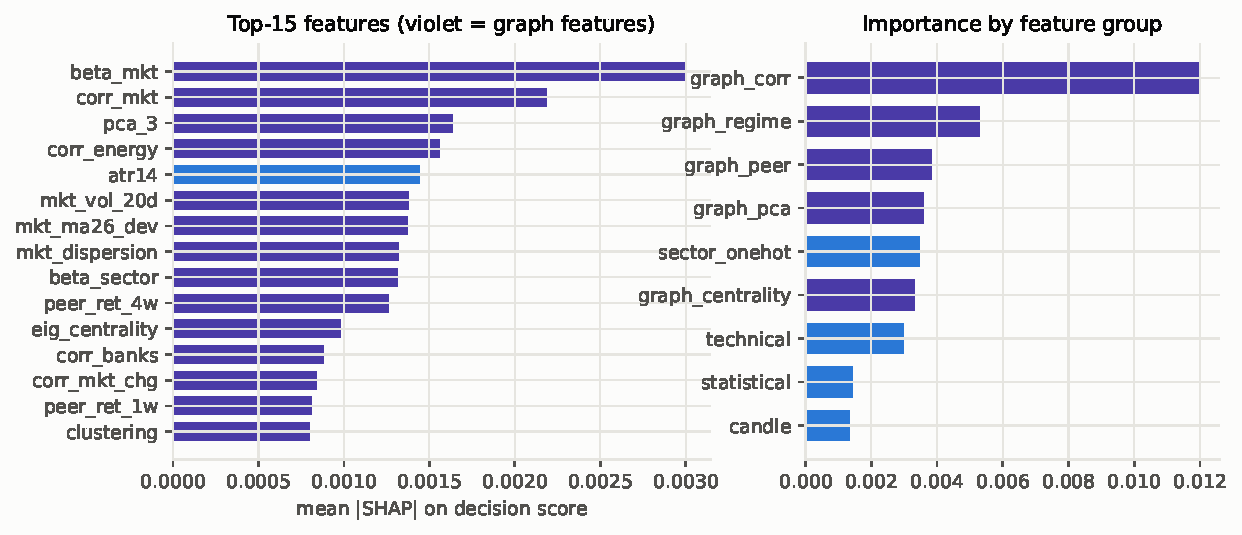
\includegraphics[width=\columnwidth]{figures/shap_importance.pdf}
\caption{SHAP (expected-gradients) attribution of the decision score. Left: top-15 features; violet bars are graph features. Right: attribution mass by feature group.}\label{fig:shap}\end{figure}
\begin{figure}[t]\centering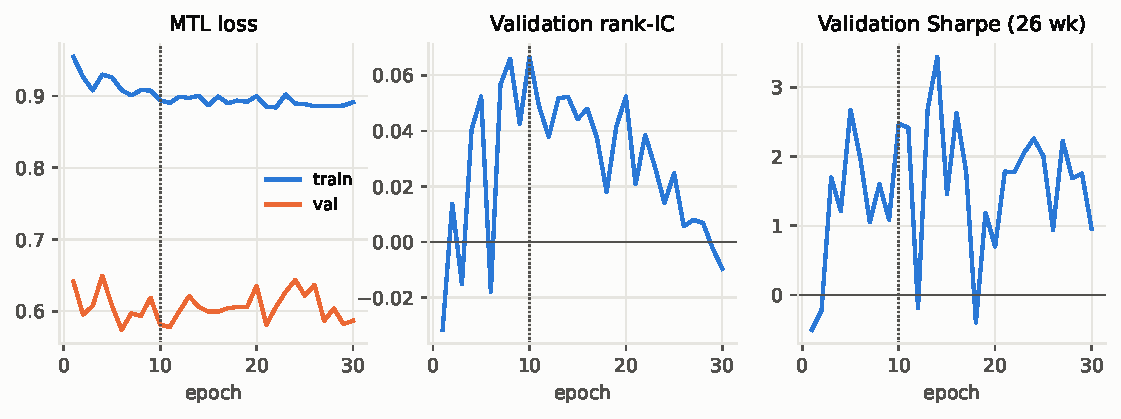
\includegraphics[width=\columnwidth]{figures/training_curves.pdf}
\caption{Training curves of the static model. The validation Sharpe (right) is far noisier than the loss or the IC; the dotted line marks the IC-selected epoch.}\label{fig:curves}\end{figure}

\textbf{Attention.} \RESULTSATT

\begin{figure}[t]\centering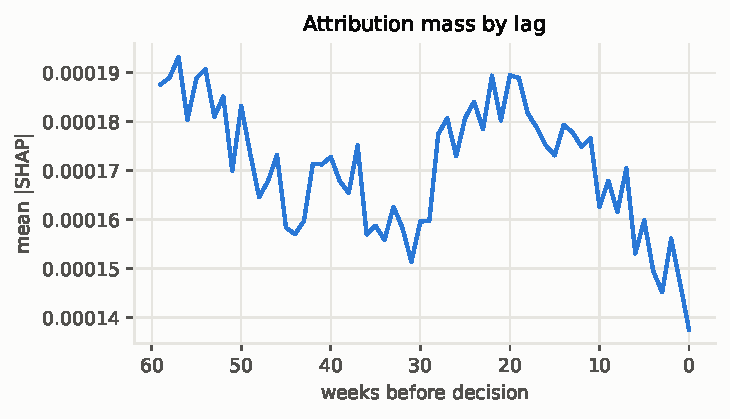
\includegraphics[width=0.8\columnwidth]{figures/shap_by_lag.pdf}\caption{SHAP attribution mass of the sequence input by lag (tuned model).}\label{fig:shaplag}\end{figure}
\textbf{Feature importance.} \RESULTSSHAP

\textbf{Decision rules.} For any recommendation the system reports predicted return, predicted volatility, score percentile and the three largest SHAP contributions; e.g.\ the \texttt{recommend} command prints ``BUY, $\hat r=+1.2\%$, $\hat\sigma=2.6\%$, score 0.46 (96th pct); factors: \ldots''. The example table produced for the first test week is in the repository (\texttt{results/tables/example\_explanations.csv}).

\subsection{Failure analysis}
\begin{table}[t]\centering\caption{Out-of-sample signal quality by market regime (buckets split at the median of each regime variable).}\label{tab:regimes}\resizebox{\columnwidth}{!}{\begin{tabular}{llrrrr}
\toprule
Regime & Bucket & Weeks & IC & $t$ & Sharpe \\
\midrule
market vol & high & 83 & 0.005 & 0.2 & 1.04 \\
market vol & low & 84 & 0.011 & 0.5 & 0.49 \\
avg correlation & high & 83 & -0.024 & -1.0 & 0.75 \\
avg correlation & low & 84 & 0.039 & 1.8 & 0.78 \\
market 12w trend & high & 83 & 0.028 & 1.3 & 1.50 \\
market 12w trend & low & 84 & -0.012 & -0.5 & 0.12 \\
dispersion & high & 83 & 0.014 & 0.6 & 0.87 \\
dispersion & low & 84 & 0.002 & 0.1 & 0.68 \\
market week & bench $<$ -2\% & 19 & 0.091 & 1.6 & -12.58 \\
market week & bench $\geq$ -2\% & 148 & -0.003 & -0.2 & 1.88 \\
\bottomrule
\end{tabular}
}\end{table}
\begin{figure}[t]\centering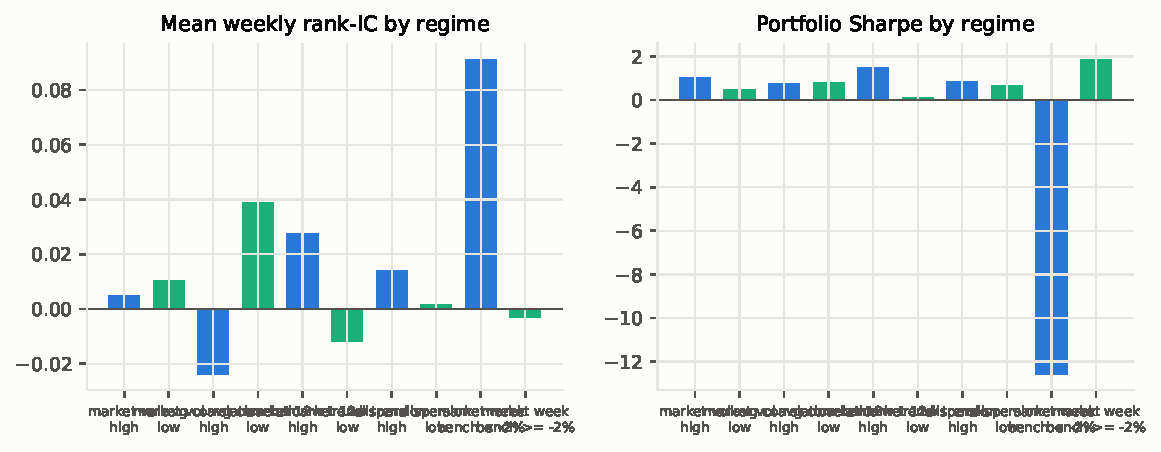
\includegraphics[width=\columnwidth]{figures/failure_regimes.pdf}\caption{Rank-IC and portfolio Sharpe by regime.}\label{fig:regimes}\end{figure}
\RESULTSFAIL

% =====================================================================
\section{Discussion and Limitations}\label{sec:limits}
\RESULTSDISC

\textbf{Limitations.} (1)~\emph{Survivorship bias}: the universe is today's Nifty~50, so stocks that were removed after poor performance are absent from training and testing; this flatters all strategies including the benchmarks built on the same universe, but not the Nifty index itself. (2)~\emph{Small universe}: with 50 names the top decile is 5 stocks, so portfolio statistics are noisy and the confidence intervals in Fig.~\ref{fig:ci} are wide. (3)~\emph{Costs}: 0.1\% per side is realistic for a retail discount broker on large caps but ignores market impact, which would matter at scale. (4)~\emph{Regime coverage}: the training window starts in 2019 and contains one crash (2020); the 2008 stress test envisaged in the PRD is impossible for many constituents that were not listed. (5)~\emph{Sector labels} are hand-curated. (6)~The test period is under four years; a Sharpe ratio measured over such a span can be positive by chance, as the intervals make explicit.

% =====================================================================
\section{Conclusion}
We built and evaluated an end-to-end recommendation engine for Nifty~50 stocks that ranks on predicted return per unit of predicted volatility, uses attention over a 60-week history together with explicit correlation-graph features, and trains with transaction costs in the objective. \RESULTSCONC{} Beyond the numbers, the work makes two practical points for applied researchers: the volatility task is where most of the learnable signal lives and it stabilizes the return task; and short-window Sharpe ratios should not be used to select models. Code and data scripts are available at the project repository.

\bibliographystyle{IEEEtran}
\begin{thebibliography}{99}\footnotesize
\bibitem{fama1993} E.~F. Fama and K.~R. French, ``Common risk factors in the returns on stocks and bonds,'' \emph{J. Financial Economics}, vol.~33, no.~1, pp. 3--56, 1993.
\bibitem{jegadeesh1993} N. Jegadeesh and S. Titman, ``Returns to buying winners and selling losers: Implications for stock market efficiency,'' \emph{J. Finance}, vol.~48, no.~1, pp. 65--91, 1993.
\bibitem{fischer2018} T. Fischer and C. Krauss, ``Deep learning with long short-term memory networks for financial market predictions,'' \emph{European J. Operational Research}, vol.~270, no.~2, pp. 654--669, 2018.
\bibitem{sezer2020} O.~B. Sezer, M.~U. Gudelek, and A.~M. Ozbayoglu, ``Financial time series forecasting with deep learning: A systematic literature review 2005--2019,'' \emph{Applied Soft Computing}, vol.~90, 2020.
\bibitem{gu2020} S. Gu, B. Kelly, and D. Xiu, ``Empirical asset pricing via machine learning,'' \emph{Review of Financial Studies}, vol.~33, no.~5, pp. 2223--2273, 2020.
\bibitem{caruana1997} R. Caruana, ``Multitask learning,'' \emph{Machine Learning}, vol.~28, pp. 41--75, 1997.
\bibitem{ruder2017} S. Ruder, ``An overview of multi-task learning in deep neural networks,'' \emph{arXiv:1706.05098}, 2017.
\bibitem{ma2021mtl} T. Ma and Y. Tan, ``Multiple stock time series jointly forecasting with multi-task learning,'' in \emph{Proc. IJCNN}, 2020.
\bibitem{engle1982} R.~F. Engle, ``Autoregressive conditional heteroscedasticity with estimates of the variance of United Kingdom inflation,'' \emph{Econometrica}, vol.~50, no.~4, pp. 987--1007, 1982.
\bibitem{bollerslev1986} T. Bollerslev, ``Generalized autoregressive conditional heteroskedasticity,'' \emph{J. Econometrics}, vol.~31, no.~3, pp. 307--327, 1986.
\bibitem{andersen2003} T.~G. Andersen, T. Bollerslev, F.~X. Diebold, and P. Labys, ``Modeling and forecasting realized volatility,'' \emph{Econometrica}, vol.~71, no.~2, pp. 579--625, 2003.
\bibitem{mantegna1999} R.~N. Mantegna, ``Hierarchical structure in financial markets,'' \emph{European Physical J. B}, vol.~11, pp. 193--197, 1999.
\bibitem{onnela2003} J.-P. Onnela, A. Chakraborti, K. Kaski, J. Kert\'esz, and A. Kanto, ``Dynamics of market correlations: Taxonomy and portfolio analysis,'' \emph{Physical Review E}, vol.~68, 2003.
\bibitem{feng2019} F. Feng, X. He, X. Wang, C. Luo, Y. Liu, and T.-S. Chua, ``Temporal relational ranking for stock prediction,'' \emph{ACM Trans. Information Systems}, vol.~37, no.~2, 2019.
\bibitem{chen2018} Y. Chen, Z. Wei, and X. Huang, ``Incorporating corporation relationship via graph convolutional neural networks for stock price prediction,'' in \emph{Proc. CIKM}, 2018.
\bibitem{vaswani2017} A. Vaswani \emph{et al.}, ``Attention is all you need,'' in \emph{Proc. NeurIPS}, 2017.
\bibitem{lundberg2017} S.~M. Lundberg and S.-I. Lee, ``A unified approach to interpreting model predictions,'' in \emph{Proc. NeurIPS}, 2017.
\bibitem{bailey2014} D.~H. Bailey, J. Borwein, M. L\'opez de Prado, and Q.~J. Zhu, ``Pseudo-mathematics and financial charlatanism: The effects of backtest overfitting on out-of-sample performance,'' \emph{Notices of the AMS}, vol.~61, no.~5, pp. 458--471, 2014.
\bibitem{politis1994} D.~N. Politis and J.~P. Romano, ``The stationary bootstrap,'' \emph{J. American Statistical Association}, vol.~89, no.~428, pp. 1303--1313, 1994.
\end{thebibliography}
\end{document}
